\documentclass[11pt]{article}
\usepackage{amsfonts}
\usepackage{amsmath}
\usepackage{graphicx}
\usepackage{amsthm}
\usepackage{Steven}
\usepackage{subfigure}

%\newtheorem{proposition}{Proposition}
\DeclareMathOperator{\var}{Var}
\DeclareMathOperator{\cov}{Cov}

\oddsidemargin -0.5in
\evensidemargin -0.5in
\textwidth 7.5in
\topmargin -0.5in
\textheight 9in

\begin{document}

\setcounter{section}{-1}
\section{Work In Progress}

\paragraph{CRLB}
Read up on the Cramer Rao Lower Bound and see how it applies to our estimator. How close is our estimator to the CRLB?

\paragraph{ENGR 361 Lecture}
Prepare 50 minute lecture on the mathematics of poker. Will also include a discussion of simpler games too.

\paragraph{ENGR 361 Homework/Recitation Worksheet}
Prepare some problems for students to do in lecture and for homework

\paragraph{Equivalent}
Reduce parallel/series subsystems to a single component that has the same probability of working. Match the mean. Reading from book borrowed from Dr. Weber.

\section{Single Link}
We consider the case where a single source is transmitting a sequence of packets to a single destination (Figure~\ref{fig:single_link}) and the source records the outcome ($X_{1}^{(n)}$ of the packet. Examples of outcomes are loss information or delay information; we consider loss based tomography. In this case, the outomes are Bernoulli random variables, with $X_{1}^{(n)}=1$ with probability $\alpha$ denoting successful reception of the packet. We are interested in developing an unbiased estimator for the link success probability $\alpha$ with a low variance.

\begin{figure}[ht!]
\centering
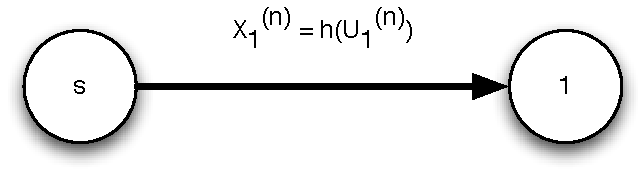
\includegraphics[width=0.4\columnwidth]{single_link}
\caption{Single Link}\label{fig:single_link}
\end{figure}

\subsection{Monte Carlo Estimation}
The simplest estimation technique is Monte Carlo. We generate a sequence of unifrom random variables $U_{1}^{(n)}$ and transforming them to Bernoulli random variables $X_{1}^{(n)} = h(U_{1}^{(n)}) = \mathbb{I}_{U_{1}^{(n)} < \alpha}$. The Monte Carlo estimator is then

\begin{equation}
\hat{\alpha}_{MC} = \frac{1}{n}\displaystyle\sum_{i=1}^{n}X_{1}^{(i)}
\end{equation}

This is clearly unbiased and has a normalized variance of

\begin{equation}
n\var\left(\hat{\alpha}_{MC}\right) = \alpha(1-\alpha)
\end{equation}

The variance as a function of $\alpha$ is shown in Figure~\ref{fig:mc}. The variance (or mean squared error) is maximum at $\alpha = \frac{1}{2}$.
\begin{figure}[ht!]
\centering
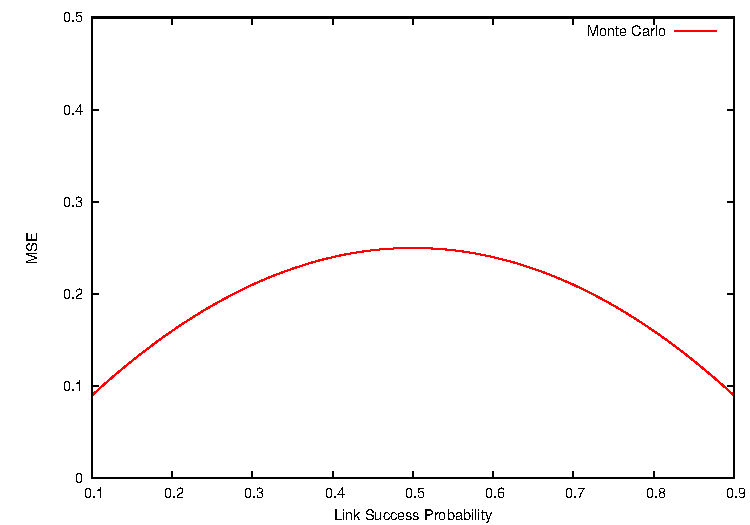
\includegraphics[width=0.75\columnwidth]{monte_carlo}
\caption{Normalized variance for Monte Carlo as a function of link success probability, $\alpha$}\label{fig:mc}
\end{figure}

\subsection{Antithetic Variables}
Our first step towards improving over the simple Monte Carlo estimation is the use of antithetic variables\cite{ross}. The idea here is that instead of generating a sequence with $n$ random variables, we generate a sequence of length $\frac{n}{2}$ and form the estimator

\begin{equation}
\hat{\alpha}_{AV} = \frac{1}{n}\displaystyle\sum_{i=1}^{n/2}h(U_{1}^{(i)})+h(1 - U_{1}^{(i)})
\end{equation}

Because expectation is linear and because $h(U_{1}^{(n)})$ and $h(1-U_{1}^{(i)})$ are identically distributed, it is easy enough to verify that the estimator is unbiased. The normalized variance is given as

\begin{align*}
n\var\left(\hat{\alpha}_{AV}\right) &= \frac{1}{n}\sum_{i=1}^{n/2}\var\left(h(U_{1}^{(i)}) + h(1-U_{1}^{(i)})\right)\\
&=\frac{\var\left(h(U_{1}^{(i)})\right) + \var\left(h(1-U_{1}^{(i)})\right) + 2\cov\left(h(U_{1}^{(i)}),h(1-U_{1}^{(i)})\right)}{2}\\
&=\var\left(h(U_{1}^{(i)})\right) + \cov\left(h(U_{1}^{(i)}),h(1-U_{1}^{(i)})\right)\\
&=\mathbb{E}\left[h(U_{1}^{(i)})^2\right] + \mathbb{E}\left[h(U_{1}^{(i)})h(1-U_{1}^{(i)})\right] - 2\mathbb{E}\left[h(U_{1}^{(i)})\right]^{2}\\
&=\alpha+ 2\mathbb{I}_{\alpha > \frac{1}{2}}(\alpha-\frac{1}{2})-2\alpha^{2}
\end{align*}

\begin{figure}[ht!]
\centering
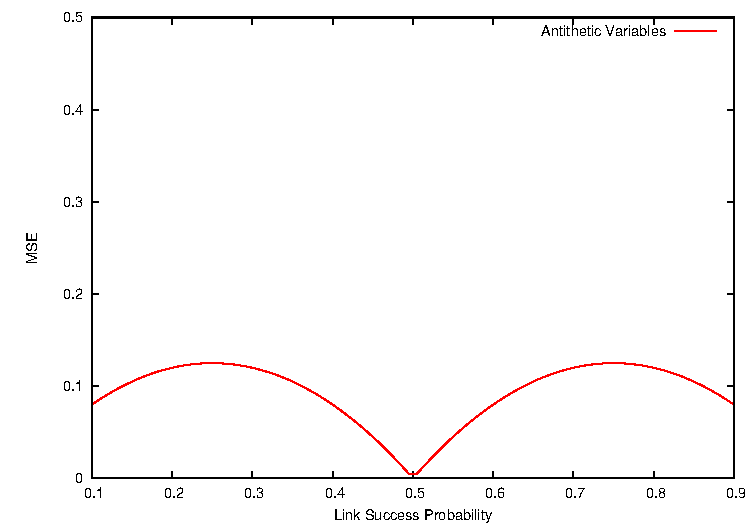
\includegraphics[width=0.75\columnwidth]{av}
\caption{Normalized variance for antithetic variables as a function of link success probability, $\alpha$}\label{fig:av}
\end{figure}

The normalized variance as a function of $\alpha$ is shown in Figure~\ref{fig:av}. Note that the normalized variance is maximum at $\alpha = \frac{1}{4}$ and $\alpha = \frac{3}{4}$. From this figure we observe:
\begin{proposition}
\[
\var\left(\hat{\alpha}_{AV}\right) < \var\left(\hat{\alpha}_{MC}\right), \forall \alpha \in (0,1)
\]
\end{proposition}

\begin{proof}
First, consider when $\alpha < \frac{1}{2}$
\[
\alpha - 2\alpha^2  <  \alpha(1-\alpha)
\]
\[
\alpha - 2\alpha^2  <  \alpha-\alpha^2
\]
\[
0  <  \alpha^2
\]
Next consider when $\alpha > \frac{1}{2}$
\[
3\alpha - 1 - 2\alpha^2 < \alpha - \alpha^{2}
\]
\[
0 < \alpha^2 - 2\alpha + 1
\]
\[
0 < (\alpha - 1)^2
\]
Finally, when $\alpha = \frac{1}{2}$ we have $\var\left(\hat{\alpha}_{AV}\right) = 0$ and $\var\left(\hat{\alpha}_{MC}\right) = \frac{1}{4}$
\end{proof}
Using antithetic variables, we have the greatest variance reduction when the variance of the Monte Carlo estimator is at its maximum. The closer $\alpha$ is to either $0$ or $1$, there is less variance reduction.

\subsection{Parameterized Antithetic Variables}
We wish to develop an estimator with a tunable parameter $\beta$ such that the variance reduction is maximized when $\beta=\alpha$, but which is an unbiased estimator for all $\alpha$ and all $\beta$.

Consider $\alpha$ fixed and unknown and to be estimated, and $\beta \in [0,1]$ chosen based on some prior assumptions about $\alpha$. Generate $U_{1}^{(n)} \sim \mathrm{Uni}(0,\beta)$ and from there set
\begin{equation}
\bar{U}_{1}^{(n)} = \frac{1-\beta}{\beta} U_1 + \beta.
\end{equation}
Note that $\bar{U}_{1}^{(n)} \sim \mathrm{Uni}(\beta,1)$. We consider an estimator of the form
\begin{equation}
\hat{\alpha}_{PAV} = \frac{1}{n} \sum_{i=1}^{n/2} \left( \beta \left( \mathbf{1}_{U_{1}^{(i)} \leq \alpha} + \mathbf{1}_{\beta-U_{1}^{(i)} \leq \alpha} \right) + (1-\beta) \left( \mathbf{1}_{\bar{U}_{1}^{(i)} \leq \alpha} + \mathbf{1}_{1-\bar{U}_{1}^{(i)} + \beta < \alpha} \right) \right)
\end{equation}
Then it is straightforward to show
\begin{eqnarray}
\Ebb[\hat{\alpha}_{PAV}] &=& \frac{1}{2} \left[ \beta \left( \Pbb(U_1 \leq \alpha) + 1 - \Pbb(U_1 \leq \beta - \alpha) \right) + (1-\beta) \left( \Pbb(\bar{U}_1 \leq \alpha) + 1 - \Pbb( \bar{U}_1 \leq 1+ \beta - \alpha) \right) \right] \nonumber \\
&=& \left\{ \begin{array}{ll}
\frac{1}{2} \left[ \beta \left( \frac{\alpha}{\beta} + 1 - \frac{\beta-\alpha}{\beta} \right) + (1-\beta) \left(0 + 1 - 1 \right) \right] , \; & \alpha \leq \beta \\
\frac{1}{2} \left[ \beta \left(1 + 1 - 0 \right) + (1-\beta) \left( \frac{\alpha-\beta}{1-\beta} + 1 - \frac{1+\beta-\alpha-\beta}{1-\beta} \right) \right], \; & \alpha > \beta 
\end{array} \right. \nonumber \\
&=& \alpha
\end{eqnarray}

We can then find the normalized variance as
\begin{equation}n\var(\hat{\alpha}_{PAV}) = \left\{
\begin{array}{llll}
(\alpha-\beta)(\beta-(2\alpha-1)), & \alpha \leq \frac{1}{2} & \beta \leq \alpha & \\
(\beta-\alpha)(2\alpha-\beta), & & \alpha < \beta \leq 2 \alpha &  \\
\alpha(\beta-2\alpha), & & \beta > 2 \alpha & \\
(1-\alpha)((2\alpha-1)-\beta), & \alpha > \frac{1}{2} & \beta \leq \alpha & \beta \leq 2 \alpha - 1 \\
(\alpha-\beta)(\beta - (2\alpha-1)), & & \beta \leq \alpha & 2 \alpha - 1 < \beta \\
(\beta-\alpha)(2\alpha-\beta), & & \beta > \alpha 
\end{array}\right.
\end{equation}

The normalized variance for both antithetic variables and parameterized antithetic variables is shown in Figure~\ref{fig:pav}.
\begin{figure}[ht!]
\centering
\subfigure[$\alpha = 0.2$]{
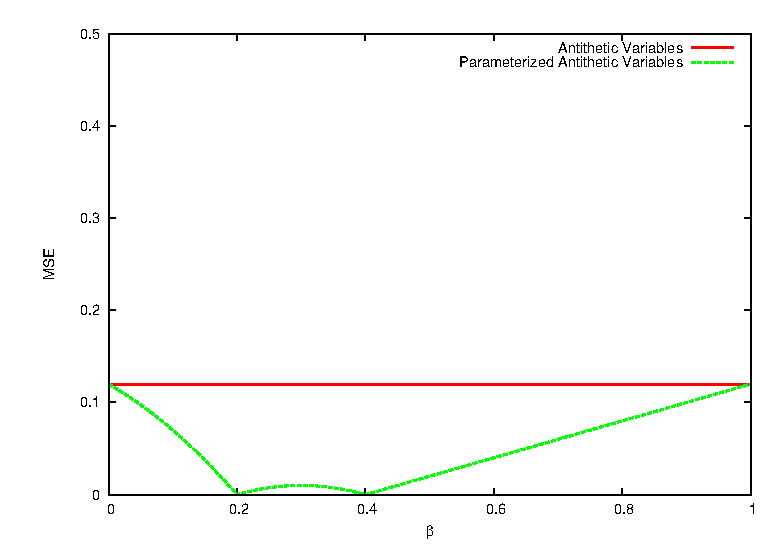
\includegraphics[width=0.4\columnwidth]{pav_2}
\label{fig:subfig1}
}
\subfigure[$\alpha = 0.4$]{
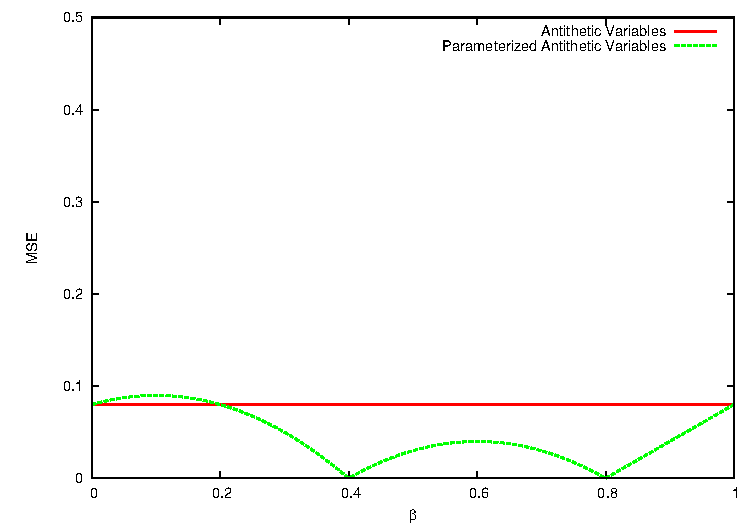
\includegraphics[width=0.4\columnwidth]{pav_4}
\label{fig:subfig2}
}
\subfigure[$\alpha = 0.6$]{
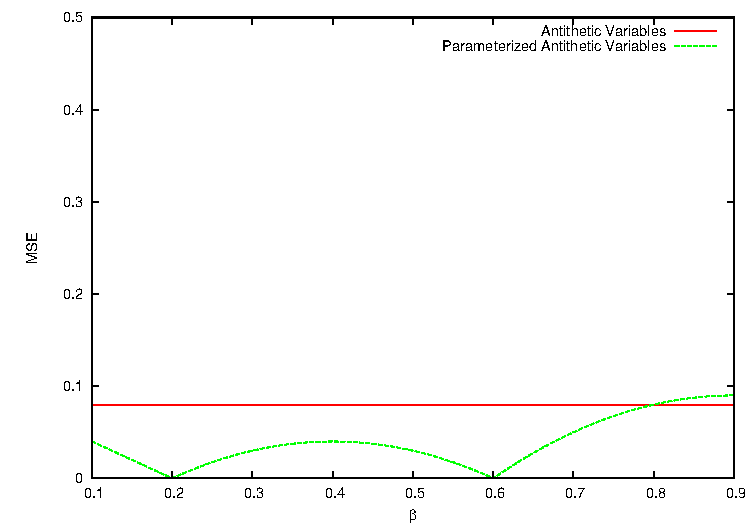
\includegraphics[width=0.4\columnwidth]{pav_6}
\label{fig:subfig3}
}
\subfigure[$\alpha = 0.8$]{
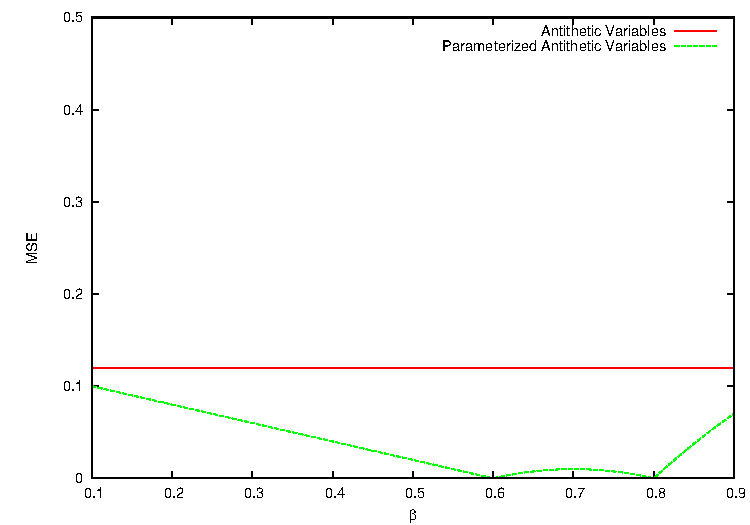
\includegraphics[width=0.4\columnwidth]{pav_8}
\label{fig:subfig4}
}
\label{fig:subfigureExample}
\caption[Normalized variance for parameterized antithetic variables]{Normalized variance for parameterized antithetic variables: \subref{fig:subfig1} $\alpha = 0.2$, \subref{fig:subfig2} $\alpha = 0.4$, \subref{fig:subfig3} $\alpha = 0.6$, and \subref{fig:subfig4} $\alpha = 0.8$}\label{fig:pav}
\end{figure}

\begin{proposition}
\[
\var\left(\hat{\alpha}_{PAV}\right) < \var\left(\hat{\alpha}_{MC}\right), \forall \alpha,\beta \in (0,1)
\]
\end{proposition}
\begin{proof}
proof goes here
\end{proof}
\begin{proposition}
If $\alpha < \frac{1}{3}$ or $\alpha > \frac{2}{3}$, then
\[
\var\left(\hat{\alpha}_{PAV}\right) < \var\left(\hat{\alpha}_{AV}\right), \forall \beta \in (0,1)
\]
\end{proposition}
\begin{proof}
proof goes here
\end{proof}

\begin{quote}
I still need to type up the propositions for the ranges of beta when alpha is in between 1/3 and 2/3 and the proposition to quantify the maximum worst case choice of beta.
\end{quote}

\section{Two Links}

\end{document}